\documentclass{book}

\usepackage{amsmath,amsthm,amssymb}
\usepackage{mathtext}

\usepackage{cmap}
\usepackage[T1,T2A]{fontenc}
\usepackage[utf8]{inputenc}
\usepackage[russian]{babel}

\usepackage[version=4]{mhchem}

\frontmatter

\title{multicorda\\Техническая документация}
\author{Денис Еманов}
\date{28.12.2022}

\begin{document}

\maketitle

\tableofcontents

\chapter{Введение}

multicorda - это небольшая операционная система, написанная на ассемблере x86 и работающая в защищённом режиме. Первая версия (v0.1) была написана в рамках курса ``Архитектура информационных систем'', читаемого на кафедре ИУ3 МГТУ имени Н. Э. Баумана.

По всем вопросам, связанным с работой multicorda, можно писать в Telegram \verb|@w1ldlight|.

Все пожелания и предложения по коду можно направлять в виде Pull Request-ов в репозиторий \verb|github.com/silentenemy/multicorda|.	

\mainmatter

\chapter{Основные особенности}

\section{Что такое multicorda}

multicorda - это миниатюрное ядро операционной системы, написанное на чистом ассемблере для архитектуры i386 и старше.

Так как это ядро уже хоть немного самостоятельной операционной системы, оно способно самостоятельно загружаться и выполнять минимальную настройку компьютера.

Кроме того, multicorda предоставляет некоторые ``библиотечные'' функции для пользовательских программ, работающих в её среде.

\section{Что может multicorda}
\begin{itemize}
\item Загружать себя с (виртуальной) дискеты;
\item Инициализировать GDT и IDT;
\item Переключать процессор в защищённый режим;
\item Перенастраивать программируемый контроллер прерываний i8259;
\item Работать с таблицами описания системы ACPI;
\item Извлекать информацию о количестве процессорных ядер;
\item Включать LAPIC;
\item Обрабатывать (некоторые) исключения процессора;
\item Получать прерывания от клавиатуры;
\item Работать с экраном.
\end{itemize}

\section{Ограничения}
\begin{itemize}
\item В настоящий момент multicorda не справляется с загрузкой с жесткого диска, только с дискеты;
\item Весь код выполняется в кольце привилегий 0;
\item В GDT есть только два перекрывающихся сегмента (кода и данных), которые покрывают 0-1 МиБ памяти;
\item В настоящий момент IOAPIC не инициализируется, поэтому работа с внешними источниками прерываний происходит через PIC 8259;
\item В настоящий момент драйвер клавиатуры может вызывать процессорные исключения.
\end{itemize}

\chapter{Установка multicorda}

\section{Тулчейн для разработки и отладки}

В качестве ассемблера используется Flat Assembler (fasm). Он был выбран за кроссплатформенность, возможность сборки бинарных файлов без заголовков ELF/PE и удобные макросы.

В качестве виртуальной машины и отладчика используется Bochs. Он позволяет отлаживать код с момента передачи управления BIOS, а также изучать полное состояние процессора и памяти в любой момент выполнения программы.

\subsection{Установка fasm}

Последнюю версию fasm можно скачать по ссылке\\ \verb|https://flatassembler.net/download.php|. Для запуска multicorda необходим fasm 1.73 или новее. 

fasm распространяется в виде zip-архива, для установки его нужно разархивировать в любую папку. Версия для Windows включает в себя небольшую IDE (fasmw.exe), в которой можно редактировать код и сразу его ассемблировать.

\subsection{Установка Bochs}

Последнюю версию Bochs (2.7) можно скачать по ссылке\\ \verb|https://sourceforge.net/projects/bochs/files/bochs/2.7/|. После установки на Windows файлы \verb|.bxrc| будут автоматически открываться в Bochs. Для запуска отладчика необходимо найти в папке установки файл \verb|bochsdbg.exe|. 

\section{Сборка multicorda}

Для сборки multicorda необходимо открыть файл \verb|main.asm| в fasmw и нажать:

\begin{center}
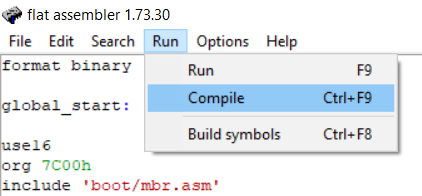
\includegraphics{pictures/2-compiling}
\end{center}

После этого в папке с исходным кодом будет создан файл \verb|main.bin|, являющийся образом дискеты для запуска multicorda.

\section{Запуск multicorda}

Примеры конфигурационных файлов для Bochs и Bochsdbg приложены к документации. Для простого запуска multicorda достаточно открыть файл \verb|.bxrc|, после чего запустится Bochs:

\begin{center}
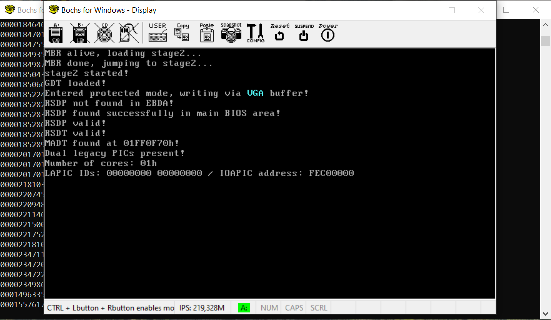
\includegraphics{pictures/2-simple-launch}
\end{center}

Для запуска дебаггера нужно запустить \verb|bochsdbg.exe| и выбрать конфигурационный файл через Load, после чего нажать Start. После этого ВМ будет ожидать запуска симуляции путем нажатия на кнопку Continue:

\begin{center}
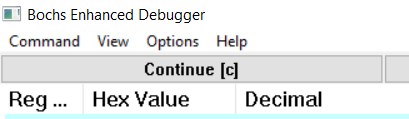
\includegraphics{pictures/2-start-debugging}
\end{center}

Также возможно использовать для запуска и отладки связку QEMU+GDB, однако это выходит за пределы данного руководства.

\chapter{Модули}

Здесь будут кратко описаны все модули multicorda и порядок их загрузки.

\section{main.asm}

Этот файл описывает порядок ассемблирования модулей и общие настройки сборки.

\section{boot/}

В этой папке расположены файлы, отвечающие за первичную загрузку кода с диска и переключение в 32-битный защищённый режим.

\subsection{mbr.asm}

Этот файл ассемблируется в первые 512 байт дискеты и считается Master Boot Record - первичным загрузчиком для этой дискеты.

\subsection{stage2.asm}

Этот файл отвечает за настройку GDT, переключение в защищённый режим и ремаппинг PIC.

\section{acpi/}

В этой папке расположены файлы, отвечающие за работу с ACPI.

\subsection{rsdp\_lookup.asm}

Этот файл описывает процесс поиска Root System Description Pointer \cite{rsdp} - указателя на Root System Description Table \cite{rsdt}, основную таблицу описания системы ACPI.

\subsection{parse\_rsdt.asm}

Этот файл описывает процесс разбора RSDT, а именно поиска таблицы Multiple APIC Description Table \cite{madt} - таблицы описания множественных APIC-контроллеров \cite{apics}. Эта таблица используется для подсчёта процессорных ядер.

\subsection{madt\_count\_cpus.asm}

Этот файл описывает процесс разбора MADT. Для каждого процессорного ядра находится его собственный Local APIC, а также находится адрес I/O APIC.

\section{interrupts/}

В этой папке расположены файлы, отвечающие за настройку IDT \cite{idt} и прерываний.

\subsection{init\_interrupts.asm}

Этот файл отвечает за инициализацию IDT и настройку обработчиков прерываний.

\subsection{enable\_apics.asm}

Этот файл отвечает за инициализацию APIC-контроллеров.

\section{lib/}

В этой папке хранятся все функции, которые можно отнести к библиотечным.

\subsection{lib/acpi/}

В этой папке хранятся файлы, необходимые для разбора заголовков RSDP и таблиц ACPI.

\subsection{lib/interrupts/}

В этой папке хранятся файлы, необходимые для инициализации IDT, работы с (A)PIC, а также базовые обработчики прерываний.

\subsection{lib/keyboard/}

В этой папке хранится код драйвера клавиатуры.

\subsection{lib/biosvga*}

Эти файлы отвечают за работу с экраном через прерывания BIOS.

\subsection{lib/memvga*}

Эти файлы отвечают за работу с экраном через видеобуфер по адресу \verb|0B8000h|.

\subsection{lib/itohex.asm}

Этот файл содержит функции для перевода целых чисел в строковый шестнадцатиричный вид.

\subsection{lib/gdt.asm}

Этот файл содержит полную таблицу GDT.

\chapter{Интересные моменты}

В процессе разработки я столкнулся с некоторыми неочевидными багами.

\section{Переход в защищённый режим}

Во время отладки перехода в защищённый режим возникла проблема, приводившая к исключению Double Fault (8h) \cite{exceptions}. Это исключение возникает в том случае, если происходит процессорное исключение во время обработки другого исключения. Double Fault является прерыванием типа Abort, после которого стабильное продолжение работы программы крайне затруднительно, а сама причина возникновения исключения обычно связана с неудачной реализацией сегментации, обработки прерываний или всего вместе. 

Я убедился в том, что GDT была написана верно, и стал отлаживать код перехода. Нюанс заключался в том, что нельзя загружать в сегментные регистры селекторы сегментов GDT до тех пор, пока не будет выставлен младший бит cr0 (бит защищённого режима) и пока не будет произведён far jump в область кода с селектором сегмента кода, например: \verb|jmp 08h:.fix_segment_registers|. Только после выполнения этих двух условий можно загружать селекторы сегментов в сегментные регистры.

\section{Ремаппинг PIC-контроллеров}

После написания обработчика прерываний клавиатуры (21h) я демаскировал прерывания PIC-контроллера и столкнулся с исключением процессора Double Fault.

Неочевидность ситуации была в том, что сообщений о первом прерывании не было. Это навело на мысль о том, что прерывание может быть не связано с реальным исключением процессора. После подробного изучения ситуации в Bochs я обнаружил, что PIT (программируемый таймер прерываний) срабатывал как раз в момент Double Fault.

Баг заключался в том, что векторы прерываний PIC-контроллеров не были перенесены на 20h-2Fh, а остались в области 8h-17h. Это было связано с тем, что процедура ремаппинга PIC-контроллеров неправильно составляла запрос, используя and вместо or для вычисления значения, передаваемого PIC-контроллеру.

\section{Настройка IDT}

Когда я реализовывал обработчики прерываний, мной был найден баг, из-за которого срабатывал только обработчики 0h и 8h (Double Fault). Ошибка заключалась в неправильном составлении IDT, а именно указатель на записи в IDT сдвигался на 64 байта, а не на 8 (длину записи).

\backmatter

\begin{thebibliography}{9}

\bibitem{fasmmanual}
  Flat Assembler 1.73 Programmer's Manual,\\
  \verb|https://flatassembler.net/docs.php?article=manual|
  (дата обращения: 28.12.2022)

\bibitem{rsdp}
  \verb|https://wiki.osdev.org/RSDP|

\bibitem{rsdt}
  \verb|https://wiki.osdev.org/RSDT|

\bibitem{madt}
  \verb|https://wiki.osdev.org/MADT|

\bibitem{idt}
  \verb|https://wiki.osdev.org/IDT|\\
  \verb|https://wiki.osdev.org/IDT_problems|

\bibitem{apics}
  \verb|https://ethv.net/workshops/osdev/notes/notes-3.html|\\
  \verb|https://wiki.osdev.org/APIC|

\bibitem{exceptions}
  \verb|https://wiki.osdev.org/Exceptions|

\end{thebibliography}

\end{document}
